\documentclass[a4paper]{article}
\usepackage[utf8]{inputenc}
\usepackage[T1]{fontenc}
\usepackage{amsmath}
\usepackage{amsfonts}
\usepackage[pdftex]{graphicx}
\usepackage[polish]{babel}
\usepackage{float}
\usepackage{mathtools}
\DeclarePairedDelimiter{\ceil}{\lceil}{\rceil}

\title{Algorytmy Równoległe – Równoległy algorytm przydziału maszyn wirtualnych oparty o branch and bound}
\author{Kamil Figiela}
\begin{document}

\maketitle

\section{Opis problemu}

Problemem do rozwiązania jest przydział maszyn wirtualnych do zadań w chmurze obliczeniowej. Dana jest lista $T$ zadań o znanym czasie wykonania $t_1..t_n$ oraz ograniczenie czasowe $D$ (deadline). Należy znaleźć taki przydział zadań do wirtualnych maszyn, aby koszt wykonania obliczenia był jak najmniejszy, oraz aby wszystkie zadania zakończyły się przed upływem terminu $D$. Zarówno koszt (złożoność) zadania jak i deadline są dodanimi liczbami rzeczywistymi. Jedna maszyna może w jednej chwili wykonywać tylko jedno zadanie, a koszt wirtualnej maszyny pobierany jest za każdą rozpoczętą godzinę jej działania, niezależnie od tego, czy jakieś zadanie jest na niej wykonywane. Wszystkie maszyny posiadają jednakową wydajność i koszt.

\section{Algorytm sekwencyjny}

Algorytm opieramy o metodę branch and bound. Na każdym poziomie drzewa decyzyjnego przypisywane jest jedno zadanie – liczba poziomów jest równa liczbie zadań. Od każdy węzeł drzewa (nie będący liściem) posiada dzieci reprezentujący przypisanie kolejnego zadania do pewnej maszyny wirtualnej. Każdy węzeł posiada liczbę dzieci o jeden większą niż liczba używanych przez już przypisane zadania maszyn – dodatkowa maszyna reprezentuje stworzenie nowej maszyny.

Rozwiązanie w danym węźle jest reprezentowane przez listę indeksów maszyn na których mają być wykonane poszczególne zadania.

\subsection{Heurystyki}

Za rozwiązanie początkowe przyjmujemy przypisanie zadań takie, że każde zadanie jest wykonywane na osobnej maszynie. Koszt takiego wykonania będzie maksymalny (upper–bound) i wynosił ($\mathop\sum\limits_{t \in T} \ceil*{t}$).

Jeżeli podczas ewaluacji danego węzła okaże się, że conajmniej jedna z maszyn przekracza deadline ewaluacja poddrzewa jest przerywana. Dodatkowo przechowujemy globalnie wartość najlepszego znalezionego rozwiązania i ucinamy poddrzewa, które przekroczą najniższy znany koszt.

Kolejną heurystyką jest obliczenie najlepszego teoretycznego kosztu ($\ceil*{\mathop\sum\limits_{t \in T} t}$). Jeżeli znajdziemy rozwiązanie o takim koszcie rezygnujemy z dalszego poszukiwania rozwiązania – lepszego już nie znajdziemy.

W celu przyspieszenia operacji ucinania poddrzew zadania sortowane są malejąco po ich koszcie – będą one przypisywane bliżej korzenia drzewa, przez co szybciej będą mogły być ucięte.

\section{Algorytmu równoległego}

Algorytm podzielono na dwie części – sekwencyjną i równoległą. Sekwencyjnie ewaluowane jest drzewo do 6 poziomu. Zadania ewaluacji kolejnych poziomów są dodawane do kolejki. Poziom 6 został wybrany arbitralnie po testach na niewielkiej próbce danych jako dający najlepsze wyniki – jego wybór steruje granularnością zadań i należy tutaj znaleźć tzw. złoty środek.

Następnie następuje część równoległa. Węzły obliczeniowe pobierają zadania z kolejki i rozpoczynają obliczenia. Po znalezieniu rozwiązania lepszego najlepsze obecnie znane węzły rozgłaszają do wszystkich informację o znalezieniu lepszego rozwiązania co poprawia skuteczność operacji ucinania poddrzew.

Jeśli zostanie znalezione najlepsze możliwe rozwiązanie wszystkie obliczenia są przerywane i program kończy pracę.

\section{Wyniki testów}

Testy zostały przeprowadzone na klastrze Zeus dla listy zawierającej 42 zadania. Ten problem jest dobrym przykładem zagadnienia dla którego zrównoleglenie może znacznie przyspieszyć obliczenia. W tym przypadku wynika to z tego, że dzięki zrównolegleniu poddrzewo zawierające bardzo dobre rozwiązanie jest przeszukiwane  równolegle z poddrzewami, które w wersji sekwencyjnej przetwarzane byłyby przed nim.

\begin{figure}[H] 
   \centering
   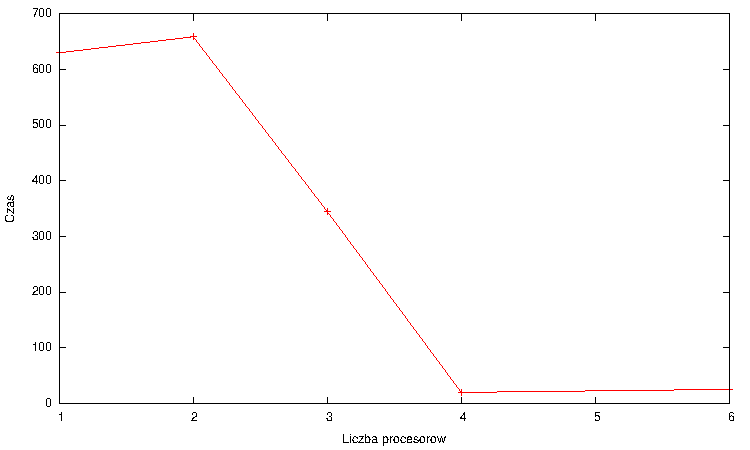
\includegraphics[width=0.7\columnwidth]{czas.pdf}
   \caption{Czasy obliczeń}
\end{figure}

\begin{figure}[H] 
   \centering
   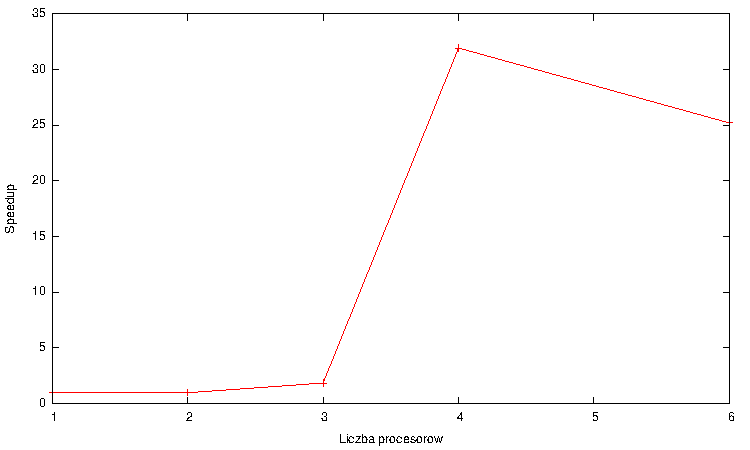
\includegraphics[width=0.7\columnwidth]{speedup.pdf}
   \caption{Speedup}
\end{figure}

\section{Dalsze prace}

\begin{itemize}
    \item Przeprowadzenie dokładniejszych testów (np. z realnymi danymi)
    \item Optymalizacja doboru poziomu drzewa na którym następuje zrównoleglanie
\end{itemize}


\end{document}

